%%%%% Don't Make Changes Below Here %%%%%
\documentclass{article}\usepackage[utf8]{inputenc}\usepackage[margin=0.4cm,top=0.4cm,bottom=0.4cm]{geometry}
\usepackage{listings}
\usepackage[usenames,dvipsnames,svgnames,table]{xcolor}\usepackage{calligra}\usepackage{tikz}\usetikzlibrary{matrix,fit,chains,calc,scopes}\usepackage{tcolorbox}\tcbuselibrary{skins}\tcbset{Baystyle/.style={sharp corners,enhanced,boxrule=6pt,colframe=Aquamarine,height=\textheight,width=\textwidth,borderline={8pt}{-11pt}{},}}\usepackage{amsmath,amssymb,amsthm,tikz,tkz-graph,color,chngpage,soul,hyperref,csquotes,graphicx,floatrow}\newcommand*{\QEDB}{\hfill\ensuremath{\square}}\newtheorem*{prop}{Proposition}\renewcommand{\theenumi}{\alph{enumi}}\usepackage[shortlabels]{enumitem}\usetikzlibrary{matrix,calc}\MakeOuterQuote{"}\newtheorem{theorem}{Theorem} \usetikzlibrary{shapes} \usepackage{lipsum}\usepackage{tabularx,ragged2e,booktabs,caption}\tcbuselibrary{breakable}\newenvironment{yframed}{\begin{tcolorbox}[breakable,colback=gray!3,title after break={\textit{\color{red}Solution (cont.)}},colbacktitle=gray!3, coltitle=black,titlerule=-1pt] }{\end{tcolorbox}}\newtcolorbox{mybox}{colback=black!15!white, colframe=white,arc=12pt}\newtcolorbox{myboxot}{colback=green!15!white, colframe=white,arc=12pt,width=120pt, height=27pt}\newtcbox{\mylib}{enhanced,boxrule=0pt,top=0mm,bottom=0mm,right=0mm,left=4mm,arc=4pt,boxsep=9pt,before upper={\vphantom{dlg}},colframe=green!50!black,coltext=green!25!black,colback=green!10!white,overlay={\begin{tcbclipinterior}\fill[green!75!blue!50!white] (frame.south west)rectangle node[text=white,font=\sffamily\bfseries\tiny,rotate=90] {Problem} ([xshift=4mm]frame.north west);\end{tcbclipinterior}}}\newtcbox{\mylibot}{enhanced,boxrule=0pt,top=0mm,bottom=0mm,right=0mm,arc=4pt,boxsep=9pt,before upper={\vphantom{dlg}},colframe=green!50!black,coltext=green!25!black,colback=green!10!white,overlay={\begin{tcbclipinterior}\fill[red!75!blue!50!white] (frame.south west)rectangle node[text=white,font=\sffamily\bfseries\tiny,rotate=90] {Other} ([xshift=4mm]frame.north west);\end{tcbclipinterior}}}
\def\Title{\begin{tcolorbox}[Baystyle,]{\begin{center}\vspace*{0.14\textheight}
{\rule{\textwidth}{1.6pt}\vspace*{-\baselineskip}\vspace*{2pt}}
\rule{\textwidth}{0.4pt}\\[0.2\baselineskip]{\fontsize{45}{45}\scshape CS 170: Efficient Algorithms and \\[-0.3\baselineskip] Intractable Problems \\[0.2\baselineskip] \calligra Spring 2017 \\[0.2\baselineskip]}
{\rule{\textwidth}{0.4pt}\vspace*{-\baselineskip}\vspace{3.2pt}}
\rule{\textwidth}{1.6pt}\\[\baselineskip]\vspace{0.05\textheight}{{\fontsize{45}{45}\scshape$\bullet$\\ {Homework 6}\\\vspace*{0.01\textheight} }{{\fontsize{18}{18}\scshape{Due on Tuesday, March 14th, 2017 at 11:59am\\}}}\fontsize{45}{45}\scshape$\bullet$  \\}\vspace*{0.1\textheight}{\fontsize{12}{12}\calligra Solutions by\\}{\fontsize{28}{28}\scshape \Name \\}\vspace*{0.01\textheight}{\fontsize{12}{12}\scshape \SID} \\\vspace*{0.05\textheight}{\fontsize{12}{12}\calligra In collaboration with\\}\vspace*{0.01\textheight}{\fontsize{12}{12}\scshape \Collabs} \\\vspace*{0.05\textheight}\end{center}}\end{tcolorbox}\newgeometry{margin=0.75in}}\def\BeginSolution{\begin{yframed}\textbf{\color{red}Solution }}\def\EndSolution{\end{yframed}}
\usepackage{algorithm}\usepackage[noend]{algpseudocode}\makeatletter\def\BState{\State\hskip-\ALG@thistlm}\makeatother\def\T{\indent}\def\star{\bigstar}
\usetikzlibrary{arrows}
\usepackage{algpseudocode}\usepackage{letltxmacro}\def\LX{\LetLtxMacro}\def\NC{\renewcommand}\LX{\oIf}{\If}\LX{\oelseif}{\ElsIf}\LX{\oElse}{\Else}\LX{\oFor}{\For}\LX{\oForAll}{\ForAll}\LX{\oRepeat}{\Repeat}\LX{\oLoop}{\Loop}\LX{\oWhile}{\While}\LX{\oFunction}{\Function}\NC{\If}[2]{\oIf{#1} #2  \EndIf}\NC{\ElsIf}[2]{\oelseif{#1} #2}\NC{\Else}[1]{\oElse #1}\NC{\For}[2]{\oFor{#1} #2 \EndFor}\NC{\ForAll}[2]{\oForAll{#1} #2 \EndFor}\NC{\Repeat}[2]{\oRepeat #1 \Until{#2}}\NC{\Loop}[1]{\oLoop #1 \EndLoop}\NC{\While}[2]{\oWhile{#1} #2 \EndWhile}\NC{\Function}[3]{\oFunction{#1}{#2} #3 \EndFunction}
\setcounter{MaxMatrixCols}{20}
%%%%% Don't Make Changes Above Here %%%%%

%%%%% Template Begins Here %%%%%

\def\Name{Ninh DO}  % Your name
\def\SID{25949105}  % Your student ID number
\def\Collabs{None} % Your collaborators here with a comma between each person's name. Write None if no collaborators. Don't leave blank.

\pagestyle{empty}
\begin{document}
\Title
%%%% Problem 1 Starts Here %%%%
\vspace{-2mm}\noindent\begin{mybox}{\begin{center}\textbf{\color{black}Problem 1: Hacking for Justice (shortcut question)}\end{center}}\end{mybox}\vspace{-2mm}
\begin{myboxot}\noindent\textbf{$\star\star\star\star\star$ Level}\end{myboxot} 

\noindent In an alternate universe, the students of CS170 found a certain problem on HW6 to be extremely difficult.
Initially, no one was able to find the solution. However, some subset of the students managed to download
the solution PDF to their laptops. These students began to send the PDF to others via email, who then sent
the PDF to others, and so on. Eventually, all of the students had the solution PDF. Uh oh!

\vspace{2pt}
\noindent After much effort, a TA has figured out the full history of the solution PDF sharing, and constructed a
directed acyclic graph $G = (V,E)$ to represent it. $V$ represents the students, and an edge $E$ from $v_1$ to $v_2$
represents that $v_1$ sent the solution file to $v_2$. All sharing is one-way, and you know that there are no cycles.

\vspace{2pt}
\noindent If the TA could go back in time, and completely block off all communications to/from one student's laptop,
which student should be blocked to minimize the number of students who received the PDF? Assume that
blocking one person will not cause anyone else to share with more people than they did before. Answer this
question in part (c), or try (a) and (b) for inspiration.

\vspace{2pt}
\noindent {\bf One more important detail}: the TA notices that for any two different paths from $A$ to $B$, the two paths
differ by at most $k$ vertices, where $k$ is a small number. You can assume $k$ is about equal to $\log(|V|+|E|)$.

\vspace{2pt}
\noindent {\bf A useful bound}: the TA also notices that if you take a depth-$k$ BFS search starting at any vertex, you will
traverse $O(k)$ vertices in the search, and the BFS search runs in $O(k)$ time. Using this property will make
the problem easier.
\begin{enumerate}
\item {\bf (10\% credit)} Is it always the case that the best student to block is one of the original students who first
downloaded the PDF? If so, explain why in 2-3 sentences. If not, give a small counterexample
\BeginSolution % 1a
% Solution Here

\EndSolution
\item {\bf(50\% credit)} Write a recursive definition for $F(s)$, the number of students that won't have the PDF if
you choose to block $s$.
\BeginSolution % 1b
% Solution Here

\EndSolution
\item {\bf(100\% credit)} Design an algorithm to determine which student to block off. Give a 4-part solution.
\BeginSolution % 1c
% Solution Here

\EndSolution
\end{enumerate}
%%%% Problem 1 Ends Here %%%%
\clearpage

%%%% Problem 2 Starts Here %%%%
\vspace{-2mm}\noindent\begin{mybox}{\begin{center}\textbf{\color{black}Problem 2: Bridge Hop}\end{center}}\end{mybox}\vspace{-2mm}
\begin{myboxot}\noindent\textbf{$\star\star\star\star$ Level}\end{myboxot} 

\noindent You notice a bridge constructed of a single row of planks. Originally there had been $n$ planks; unfortunately,
some of them are now missing, and you're no longer sure if you can make it to the other side. For convenience, you define an array $V[1\ldots n]$ so that $V[i]$ = \textsc{True} iff the $i$th plank is present. You're at one side of the bridge, standing still; in other words, your {\it hop length} is 0 planks. Your bridge-hopping skills are as follows: with each hop, you can increase or decrease your hop length by 1, or keep it constant.

\hspace*{-0.5cm} 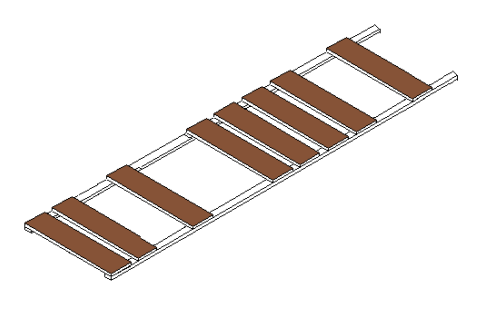
\includegraphics[width=2in]{bridge}

\vspace{2pt}
\noindent For example, the image above has planks at indices $[1, 2, 4, 7, 8, 9, 10, 12]$, and you could get to the other
side with the following hops: $[0, 1, 2, 4, 7, 10, 12, 14]$.

\vspace{2pt}
\noindent Clarifications: You start at location 0, just before the first plank. Arriving at any location greater than $n$
means you've successfully crossed. Due to your winged shoes, there is no maximum hop length. But you can only hop forward (hop length cannot be negative).

\vspace{2pt}
\noindent Devise an efficient algorithm to determine whether or not you can make it to the other side.

\vspace{2pt}
\noindent For this problem, you should know how to do the proof of correctness, but need not include it in your
submission. You should submit the main idea, pseudocode, and runtime.

\BeginSolution % 2
\\
\underline{\textbf{Main idea:}}\\
Imagine that we are at the i-th plank of the bridge and we have just made an l-plank hop. We want to check if there is any plank in next (l-1)-plank, l-plank or (l+1)-plank hop. Therefore, if the problem is BridgeHop(l, i) asking if we can make it to the other side from the i-th plank, it turns into three subproblems BridgeHop(l-1, i+l-1]), BridgeHop(l, i+l]) and BridgeHop(l+1, i+l+1]), where V[i+l-1], V[i+l], V[i+l+1] are True's IF these planks exist. If any of these planks does not exist, we just simply omit the subproblem. If all of these three planks do not exist, we return false immediately.\\
Using dynamic programming, we start with 1-plank hop from the beginning of the bridge and call the function recursively with the current plank position.\\
\underline{\textbf{Pseudocode:}}\\
%
\begin{lstlisting}
for i in range(len(V), 2*len(V)):
	V.append(True)
for i in range(len(V)):
	for j in range(0, 2*len(V)):
		cache[i][j] = None
print(BridgeHop(0,0))

def BridgeHop(l, i):
	if i >= n+1:
		return True
	else:
		if cache[l][i] != None:
			return cache[l][i]
		else:
			ret = V[i] and (BridgeHop(l-1, i+l-1) or \
				BridgeHop(l, i + l) or BridgeHop(l+1, i+l+1))
			cache[l][i] = ret
			return ret
\end{lstlisting}
%
\underline{\textbf{Runtime:}}\\
Without using cache, the runtime would be $O(3^n)$ but with using cache, the runtime will depend on the size of cache which is $O(n^2)$
\EndSolution


%%%% Problem 2 Ends Here %%%%
\clearpage

%%%% Problem 3 Starts Here %%%%
\vspace{-2mm}\noindent\begin{mybox}{\begin{center}\textbf{\color{black}Problem 3: Longest Palindrome Substring}\end{center}}\end{mybox}\vspace{-2mm}
\begin{myboxot}\noindent\textbf{$\star\star\star\star$ Level}\end{myboxot} 

\noindent A substring is {\it palindromic} if it is the same whether read left to right or right to left. For example, "bob" and "racecar" are palindromes, but "cat" is not. Devise
an algorithm that takes a sequence $x[1\ldots n]$ and returns the length of the longest palindromic substring. Its running time should be $O(n^2)$.

\vspace{2pt}
\noindent For this problem, you should know how to do the proof of correctness, but need not include it in your
submission. You should submit the main idea, pseudocode, and runtime.

\BeginSolution % 3
\\
\underline{\textbf{Main idea:}}\\
Check both ends of the substring, if they are identical characters, the length of the palindrome P in the string S is len(P in S) = 2 + len(P[1:end-1] in S[1:end-1]), where P[1:end-1] , S[1:end-1] are the substrings of P, S truncated at both ends, respectively. If they are not identical, the palindrome must lie either in S[1:] or S[:end-1], so len(P in S) = max(len(P in  S[1:]), len(P in S[:end-1]). We use dynamic programming.\\
Similar to the previous problem, in order to reduce the runtime we use cache to avoid duplicated calculation.\\
\underline{\textbf{Pseudocode:}}
%
\begin{lstlisting}
for i in range(len(S)):
	for j in range(len(S)):
		cache[i][j] = None

def LenOfPalind(i,j,S):
	if len(S) == 0:
		return 0
	elif len(S) == 1:
		return 1
	else:
		if S[0] == S[end]:
			if cache[i][j] != None:
				return cache[i][j]
			else:
				ret = 2 + (i+1, j-1, S[1:end-1])
				cache[i][j] = ret
				return cache
		else:
			if cache[i][j] != None:
				return cache[i][j]
			else:
				ret = max(LenOfPalind(i+1,j,S[1:]), \
					LenOfPalind(i,j-1,S[:end-1]))
				cache[i][j] = ret
				return ret
\end{lstlisting}
%
\underline{\textbf{Runtime:}}\\
In worst case, the runtime is the time to fill the array cache which is $O(n^2)$
\EndSolution
%%%% Problem 3 Ends Here %%%%
\clearpage

%%%% Problem 4 Starts Here %%%%
\vspace{-2mm}\noindent\begin{mybox}{\begin{center}\textbf{\color{black}Problem 4: A Sisyphean Task}\end{center}}\end{mybox}\vspace{-2mm}
\begin{myboxot}\noindent\textbf{$\star\star\star\star$ Level}\end{myboxot} 

\noindent Suppose that you have $n$ boulders, each with a positive integer weight $w_i$. You'd like to determine if there is any set of boulders that together weigh exactly $k$ pounds. You may want to review the solution to the
Knapsack Problem for inspiration.

\vspace{4pt}
\noindent For this problem, you should know how to do the proof of correctness, but need not include it in your
submission. You should submit the main idea, pseudocode, and runtime.

\begin{enumerate}
\item Design an algorithm to do this.
\BeginSolution % 4a
\\
\underline{\textbf{Main idea:}}\\
We want to know if there are any number of boulders among n ones summing up to $k$ pounds. Take an arbitrary weight $w_i$, there are two scenarios:
%
\begin{enumerate}[1.]
	\item Some boulders among the remaining $n-1$ boulders sum up $k$ pounds.
	\item Some boulders among the remaining $n-1$ boulders sum up $k - w_i$ pounds
\end{enumerate}
%
Thus, the recursive equation looks like:\\
	$Sum(n,k) = Sum(n-1,k)\ or\ Sum(n-1,k-w_i)$
We use dynamic programming. The main problem will recurse to the base case problems. If k drops below 0, return false. If k == 0, then it will be false if we still have weight(s), or true if we do not have any weight left.\\
\underline{\textbf{Pseudocode:}}\\
%
\begin{lstlisting}
for i in range(n):
	for j in range(k):
		cache[i][j] = None

def Sum(n,k,W):
	if n == 0:
		if k != 0:
			cache[n][k] = false
			return false
		else:
			cache[n][k] = true
			return true
	else:
		if k < 0:
			cache[n][k] = false
			return false
		for i in range(n):
			ret = Sum(n-1,k-W[i],W) or Sum(n-1,k,W)
			cache[n][k] = ret
			return ret
\end{lstlisting}
%
\underline{\textbf{Pseudocode:}}\\
Again, the strategy is to use cache to reduce the runtime into the time to populate cache which is O(nk)
\EndSolution

\item Is your algorithm polynomial in the {\it size} of the input? Remember that size is in terms of how many bits we need.
\BeginSolution % 4b
\\
NO. The algorithm does not mention anything about the size of the input. It is proportional to $k$ which is the magnitude of the input rather than the size of the input which is the number of bits or logarithm of the magnitude.
\EndSolution
\end{enumerate}
%%%% Problem 4 Ends Here %%%%
\clearpage

%%%% Problem 5 Starts Here %%%%
\vspace{-2mm}\noindent\begin{mybox}{\begin{center}\textbf{\color{black}Problem 5: Advertising Network}\end{center}}\end{mybox}\vspace{-2mm}
\begin{myboxot}\noindent\textbf{$\star\star\star\star\star$ Level}\end{myboxot} 

\noindent You are an advertising network tasked with making bids on Facebook's mobile ad units for your customers.
On each day, you make a bid of $\$\theta, \theta \in [0,1]$, and win that day's auction with probability $\theta$. If you don't win, then you don't spend any money. As per your contract with your customers, you {\it need} to win at least $k$ out of $n$ auctions that will occur this fiscal year.

\vspace{4pt}
\noindent An obvious approach may be to bid $\$1$ for each of the first $k$ days, then nothing for the rest of the $n$ -- $k$ days --- this strategy will cost you $\$k$. However, it may not be optimal! Consider this alternative for $n = 30, k = 4$:
\begin{itemize}
\item Bid $\$0.50$ for each of the first 26 days, or until you've won 4 auctions.
\item Bid $\$1.00$ for each of the next 4 days, if you didn't win them yet.
\item This strategy will have expected cost $\$2.00$ (round to the nearest cent), and worst case cost $\$4.00$ -- a strictly superior strategy.
\end{itemize}
\vspace{4pt}
\noindent Give an optimal strategy to minimize expected cost while maintaining your contract, for any $k, n$. You only need to explain the main idea; no need for proof, runtime, or pseudocode.

\vspace{4pt}
\noindent Here are some hints:
\begin{itemize}
\item You'll need to use probability; specifically, the linearity of expectation.
\item Parameterize your strategy as a set of variables $\theta_{n, k}$, and notice that you need to minimize some function that can be written in terms of $\theta_{n, k}$.
\item To actually solve said optimization problem, you can assume you have access to a quadratic program solver that can minimize any quadratic function of a single variable, in time that is efficient.
\end{itemize}
\BeginSolution % 5
\\
Given $n$ days and $k$ bid wins, we have to minimize the expected cost $E[n,k]$. There are two scenarios:
%
\begin{enumerate}[1.]
	\item We win today with the probability $\theta_{n,k}$, we pay $\theta_{n,k}$. The expected cost becomes $\theta_{n,k} + E[n-1,k-1]$
	\item We lose today with the probability $1 - \theta_{n,k}$, we pay nothing. The expected cost becomes $E[n-1,k]$
\end{enumerate}
%
We come up with the recursive equation for the expected cost:
%
\begin{equation}
E[n,k] = \theta_{n,k}\left(\theta_{n,k} + E[n-1,k-1]\right) + \left(1 - \theta_{n,k}\right)E[n-1,k]
\end{equation}
%
The equation recurses the expected cost $E[n,k]$ to two base cases which are:
%
\begin{equation}
E[i,i] = i \qquad \text{and} \qquad E[j,0] = 0
\end{equation}
%
for whatever $i\leq k$ and $j\leq n-k$.\\
With dynamic programming, the problem $E[n,k]$ turns into the subproblems $E[n-1,k]$ and $E[n-1,k-1]$. When it hits the base cases, we can use the quadratic program solver to minimize the expected cost that takes the form of a quadratic function. In each recursion call, the quadratic program solver is applied to minimize the return until it gets back to the main problem. 
\EndSolution
%%%% Problem 5 Ends Here %%%%
\clearpage

%%%% Problem 6 Starts Here %%%%
\vspace{-2mm}\noindent\begin{mybox}{\begin{center}\textbf{\color{black}Problem 6: Knightmare (extra credit question)}\end{center}}\end{mybox}\vspace{-2mm}
\begin{myboxot}\noindent\textbf{$\star\star\star\star\star\star$ Level}\end{myboxot} 

\noindent Give an algorithm to find the number of ways you can place knights on an $N$ by $M$ chessboard such that no two knights can attack each other (there can be any number of knights on the board, including zero knights). The runtime should be $O(2^{3M}\cdot N)$ (or symmetrically, switch the variables).

\vspace{4pt}
\noindent Note that even though this question is extra credit (and thus only worth 1 pt), the staff {\it strongly recommends} that you at least attempt it and understand the solution. It will be {\it very} helpful practice for your upcoming midterm, which we remind you will be Monday March 20, 2017.

\BeginSolution % 6

\EndSolution
%%%% Problem 6 Ends Here %%%%
\clearpage

\end{document}
%%%%% Template Ends Here %%%%%














